\begin{problem}{범죄자}
	{standard input}{standard output}
	{3 seconds}{128 megabytes}{}
	
	지구이웨는 강을 낀 아름다운 마을이다. 강가에는 $n$개의 집이 있고, 상류에서 하류까지 1부터 $n$까지 번호가 붙은 집들이 있다. 지구이웨는 조용하고 모두가 행복한 마을이었다. 하지만 최근에 두 위험한 범죄자인 범수와 상수가 마을에 나타났다. 그들은 이미 도둑질을 많이 해서 사람들은 집을 나가는것도 무서워 했다.
	
	범수와 상수가 하는 도둑질은 단순하지 않고, 전체 집을 도둑질 한다. 하나의 집을 나오면, 서로를 향해 걸어가고 뒤로 돌아가지는 않는다. 범수는 하류쪽으로(숫자가 큰 쪽으로), 상수는 상류쪽으로(숫자가 작은 쪽으로) 걸어간다. 길을 걷는 동안, 서로가 만나기 전에는 각자가 몇몇 집으로 들어가서 물건들을 훔친다. 그 후에 그들은 집에서 만나서 그들이 훔친 물건들을 나눠갖는다. 지구이웨 주민들은 현기증이 났다. -- 그들의 평화를 되찾아야 한다! 그래서 탐정 사과에게 도움을 요청했다.
	
	형사는 도둑이 같은 색의 집에 살고 있지만 어떤 사람인지는 모른다고 판정했다. 방금 익명의 사람이 도둑들이 급습중이라고 밝혔다. 소식통은 자신의 안전을 두려워해서, 어떤 집으로 들어갈지 밝히지는 않았다. 하지만 그들의 색은 밝혔다. 또한, 도둑들은 한 종류의 색의 집을 한 번만 도둑질 할 것이라는 미신을 가지고 있다.
	
	사과는 더 이상 기다릴 수 없다. 그는 도둑들이 만나는 장소에서 잠복할 것이다. 도둑들이 모이는 것이 가능한 장소를 모두 찾는 프로그램을 작성하여라.
	
	
	\InputFile
	
	첫째 줄에는 집의 수를 의미하는 정수 $n$과 지구이웨에 있는 집의 색의 수를 의미하는 정수 $k$가 공백 하나로 구분되어 주어진다. ($3 \le n \le 1,000,000$, $1 \le k \le 1,000,000$, $k \le n$) 둘째 주렝는 $n$개의 정수로 이루어진 수열 $c_1, c_2, \cdots, c_n$ ($1 \le c_i \le k$)가 공백 하나로 구분되어 주어진다. 이 수는 지구이웨에 있는 집들의 숫자들을 나열해 놓은 것이다.
	
	셋째 줄에는 범수와 상수가 들어갈 집의 갯수를 나타내는 $m$, $l$이 공백 하나로 구분되어 주어진다. ($1 \le m, l \le n$, $m+l \le n-1$)
	넷째 줄에는 $m$개의 정수 $x_1, x_2, \cdots, x_m$이 공백 하나로 구분되어 주어지고, 범수가 (자신의 집을 제외하고) 들어갈 집의 색을 차례로 나타낸다. ($1 \le x_i \le k$)
	다섯째 줄에는 $l$개의 정수 $y_1, y_2, \cdots, y_l$이 공백 하나로 구분되어 주어지고, 상수가 (자신의 집을 제외하고) 들어갈 집의 색을 차례로 나타낸다. ($1 \le y_i \le k$)
	$x_m = y_l$이고, 이 수는 범수와 상수가 자신이 도둑질한 물건들을 나눌 장소를 나타낸다. (그들은 그 집도 도둑질 할 것이다.)
	
	\OutputFile
	
	당신의 프로그램은 두개의 줄을 출력해야 한다. 첫째 줄은 위의 조건을 만족하면서 만날 수 있는 집의 갯수를 출력하여야 한다. 둘째 줄은 두 명이 만날 수 있는 집의 번호를 오름차순으로 출력해야 한다. 만약 상수와 범수가 만날 수 없다면, 첫째 줄은 0이어야하고, 둘째 줄은 비어있어야 한다.
	
	\Examples
		
	\begin{example}
	\exmp{
15 7
2 5 6 2 4 7 3 3 2 3 7 5 3 6 2
3 2
4 7 3
5 3
	}{%
3
7 8 10
	}%
	\end{example}
	
	\Notes
	
	\begin{center}
		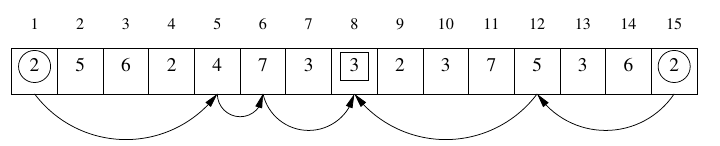
\includegraphics[width=1.0\linewidth]{prz.png}
	\end{center}
	
	위의 예제에서, 도둑들은 2번 색 (범수가 1번 혹은 4번 집, 상수가 15번 집) 혹은 6번 색 (범수가 3번 집, 상수가 14번 집)의 집에 살고 있을 것이다. 범수는 5번 집 (4번 색), 6번 집 (7번 색)을 차례로 들어가고 7번, 8번, 10번 집 (3번 색) 중의 하나에 들어갈 것이다. 상수는 12번 집 (5번 색)을 들어가고 7번, 8번, 10번 집 (3번색) 중의 하나에 들어갈 것이다. 위의 그림은 범수가 1번집에 살고, 도둑들이 8번 집에서 모이는 상황을 나타낸다.
	
\end{problem}

